\chapter{Research Design and Method}

\label{ch:method}

This chapter describes what was built, what it was tested on and how it was evaluated.
It covers the evaluation method, the pipeline, the benchmark and its two splits, four linking methods, the linking ground truth, the execution environment and metrics, the prompt interventions, the recovery methods, and the models and reproducibility procedures.

\section{Stage-Wise Diagnostic
Evaluation}

Text-to-SPARQL systems are usually evaluated end to end, with one score per system that shows how useful it is but says little about why it fails: one system may identify every entity correctly but build the wrong structure, another may get the structure right but use a wrong identifier, and both end up with the same score for different reasons.
The underlying process can nonetheless be split into component decisions (entity detection, entity linking, relation selection and query construction)~\citep{mohammed2018strong}, and this is what makes stage-wise measurement possible.

This thesis uses stage-wise diagnostic evaluation, a four-step protocol (\cref{fig:method}).

\textbf{First, intermediate ground truth is derived from artefacts the benchmark already provides.}
Instruct-to-SPARQL contains each query twice, once with identifiers and once with those identifiers replaced by labels; since the two versions are aligned position by position, they yield mention-level linking ground truth without additional annotation, and the same approach works for any benchmark that provides aligned gold and label-form queries.

\textbf{Second, the stage of interest is isolated by keeping all other stages fixed.}
Each condition changes only one component and reuses the same generated queries, candidate pools, execution environment and scoring; where possible, the varied stage also receives its gold value, which creates an upper-bound condition (not itself a performance claim) whose difference from the full pipeline estimates the error attributable to that stage.

\textbf{Third, the remaining error is attributed and checked against independent evidence.}
Simple subtraction is not enough, because the unexplained remainder may have several causes, so the subtraction-based attribution is compared with a manually annotated failure sample, corpus-wide construct counts and agreement between independent systems; the attribution is reported with the confidence interval that the weakest evidence supports, and disagreements between sources are reported as well.

\textbf{Fourth, the proposed cause is tested through intervention.}
If a system lacks particular knowledge, supplying it should improve performance, and the size of the improvement shows how much error the missing knowledge explains.
Interventions that do not help are still informative, because they narrow down the explanations for the observed errors; the next chapter reports all of them alongside the one that works.

The protocol is defined independently of the specific pipeline used here.

\begin{figure}[htbp]
  \centering
  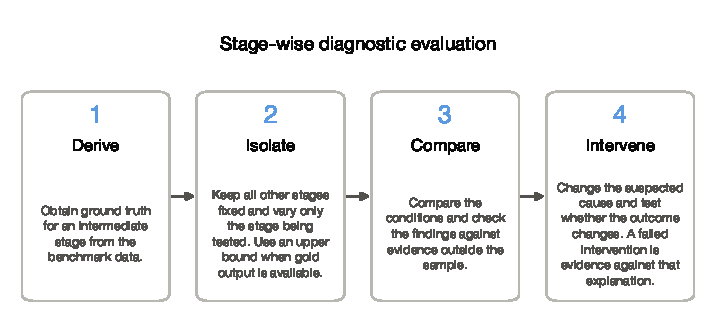
\includegraphics[width=0.88\textwidth]{figures/fig_method.pdf}
  \caption{\Method{}: the four moves.}
  \label{fig:method}
  \tabnote{The protocol is independent of the pipeline and can
be applied to other benchmarks that provide aligned gold and label-form
queries.}
\end{figure}

\section{Pipeline Architecture}

\label{sec:method-framework}

The system is a modular pipeline built on frozen language models, and no stage uses fine-tuning.
It follows the pipeline paradigm described in the previous chapter, with fixed stages and observable intermediate outputs instead of a single sequence-to-sequence model or an open-ended agent.
This design was chosen mainly with diagnosis in mind: named stages can be measured, replaced and given gold values one at a time, as the diagnostic protocol requires.

\paragraph{The Six Stages}

For each question, the pipeline runs the following steps.
\Cref{fig:pipeline} shows the complete arrangement and the two evaluation conditions.

\textbf{1.\ Labelled-query generation.}
The model receives a system prompt that asks it to act as a Wikidata SPARQL expert and write a query that answers the question.
Instead of opaque identifiers, it must use human-readable labels in a fixed bracket format: wd:[entity:LABEL] for entities and wdt:[property:LABEL] for properties.
It is told to keep ordinary SPARQL structure and to output only the query.
Decoding is deterministic, and Markdown code fences are removed.
The notation comes from the benchmark itself.
\textcite{xu2023wikisp} use a similar label-based representation, as do \textcite{banerjee2023gettqa}, whose grounding step based on graph embeddings performs a comparable substitution from labels to identifiers.
Using the benchmark's notation means that generated and reference queries can be compared in the same vocabulary.

\textbf{2.\ Label parsing.}
Regular expressions extract the entity and property labels from the generated query.
Duplicate labels are removed, and the original order is kept.

\textbf{3.\ Candidate retrieval.}
For each label, the top seven candidates are retrieved from Wikidata's wbsearchentities API.
Entity labels are searched among items and property labels among properties.
Each candidate comes with an identifier, a label and a short description.

When requests arrive too quickly, the API can silently return empty results, which makes throttling hard to tell apart from a label that has no matching candidate.
To reduce this problem, requests are rate-limited and candidate pools combine repeated retrievals.
Empty results are requested again until the pools are stable.

\textbf{4.\ Disambiguation.}
Each label is mapped to one candidate identifier.
This is the stage that the linker comparison varies, and the four implementations are described below.
All other stages stay the same, so the comparison concentrates on the disambiguation mechanisms.

\textbf{5.\ Substitution.}
The selected identifiers replace the labels in the query.
A query counts as fully linked only when no bracket placeholder remains.
Partial substitution is recorded as a linking failure and is not passed on to execution.

\textbf{6.\ Execution and scoring.}
The substituted query is executed against the endpoint, and its result set is compared with the reference result set.
The execution environment and the scoring metric are described later in this chapter.
For each question, the pipeline records whether a labelled query was generated, whether all labels were linked and whether the query executed.
These indicators make the stage analysis in the results chapter possible.

\paragraph{Three Decisions}

Translating a question into a query involves three decisions.
\emph{Concept selection} decides which entities and properties the query needs.
\emph{Structural composition} arranges them with Wikidata's constructs, such as statement nodes, qualifiers, class closure and aggregation.
\emph{Disambiguation} decides which identifier a given label denotes, among the retrieved candidates.
In this pipeline the generator makes the first two decisions when it writes the labelled query, and the linking stage makes the third.
In this thesis, \emph{linking} refers to the third decision, the mapping from a label to its identifier.

\paragraph{Two Conditions}

The pipeline is evaluated under two conditions, and the difference between them is the upper-bound construction described above.

In the \textbf{gold-label condition}, generation is skipped and the labels come from the benchmark's annotated query.
Concept selection and query structure are therefore correct by construction, and only disambiguation is evaluated.
Comparing this condition with the full pipeline estimates the error caused by generating the query, that is, by concept selection and structural composition together.

In the \textbf{end-to-end condition}, the model generates the labelled query and the same linking stages follow.
This condition represents the deployed system and provides the main pipeline results.

One design asymmetry needs mentioning.
Property labels are resolved with the reasoning-based method in every condition, including those in which other linkers resolve the entities, because none of the compared systems links Wikidata properties.
As a side benefit, entity-linking and property-linking errors can be measured separately, in line with \textcite{scharpf2026survey}, who identify joint entity and predicate linking as an underdeveloped area.
The split is a diagnostic design choice, not a claim that the two tasks are best solved independently: joint entity--relation linking is an established alternative that exploits the compatibility between candidate entities and relations~\citep{dubey2018earl}.

\begin{figure}[htbp]
  \centering
  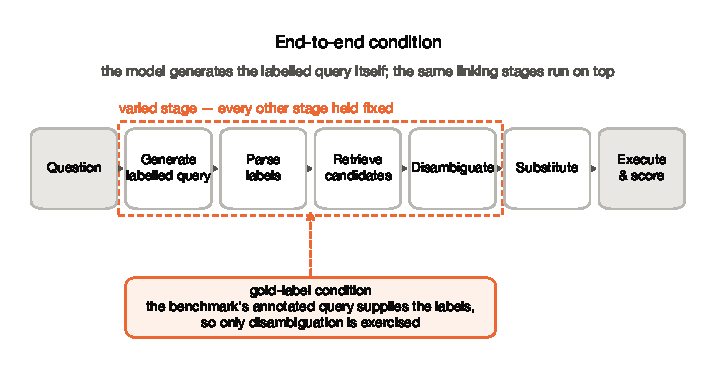
\includegraphics[width=0.88\textwidth]{figures/fig_pipeline.pdf}
  \caption{Pipeline architecture and the two evaluation conditions.}
  \label{fig:pipeline}
  \tabnote{The pipeline has six stages. In the gold-label
condition, the benchmark's annotated query supplies the labels, so
generation is skipped. All other stages remain identical.}
\end{figure}

\section{Benchmark and Experimental
Conditions}

\label{sec:method-pipeline}
\label{sec:setup-benchmark}

The benchmark is Instruct-to-SPARQL~\parencite{benamor2025instruct}.
It pairs natural-language instructions with executable Wikidata queries and assigns complexity labels.
It was chosen for three reasons.
First, its queries were collected from tutorial and example pages instead of being generated from templates, so they reflect the modelling conventions of actual Wikidata users.
Second, its complexity labels make it possible to see where systems fail.
Third, and most important here, each query is provided both with identifiers and with those identifiers replaced by human-readable labels, which enables the ground-truth derivation described below.

\paragraph{Two Splits, Two Jobs}

Two evaluation splits serve different purposes.
The \textbf{working split} was created from the released data with complexity stratification, a fixed seed and a 75/5/20 train-validation-test division, keeping one natural-language instruction per query.
Its test set contains 567 queries (38 simple, 222 medium, 307 complex) and is used for the diagnostic analysis: the stage table, error taxonomy, construct analysis, prompt interventions and cascade.
The \textbf{official split} is the benchmark authors' own test split, used for the comparison with their published systems.
Each experiment uses the split that fits its purpose and no result is reported twice, with one exception: the linker comparison is replicated on both splits to test whether it depends on the split chosen; differences in row counts are explained where they occur.

\begin{figure}[htbp]
  \centering
  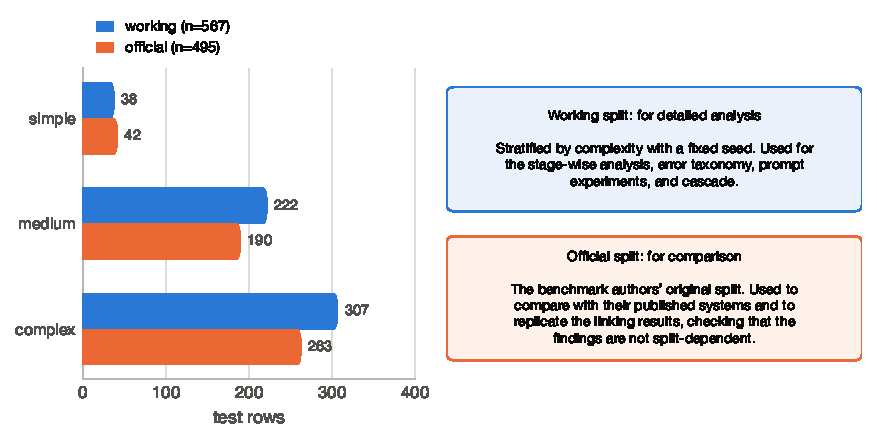
\includegraphics[width=0.88\textwidth]{figures/fig_splits.pdf}
  \caption{The two-split design.}
  \label{fig:splits}
  \tabnote{The splits have different purposes and are not
interchangeable. Only the linker comparison uses both splits, allowing
the stability of its ordering to be examined.}
\end{figure}

\paragraph{Dataset Drift}

The dataset's identifier field is not stable between the raw file used to build the working split and the current release.
Some identifiers point to different questions in the two versions, so rows are matched on normalised instruction text instead.
The release offers two configurations with different splits; the official-split experiments use the default configuration, whose 495 test rows match the benchmark paper (the with-limit configuration has 493).
Against the default configuration, 365 of the 567 working test rows (64.4\%) correspond to official training rows, 95 (16.8\%) to official test rows and 24 (4.2\%) to validation rows, 6 (1.1\%) have instructions that occur in more than one official split, and 77 (13.6\%) have no counterpart; the revision used here is pinned in the repository.
This overlap does not contaminate the results of this thesis, since none of the models is fine-tuned on the benchmark; it matters only for the comparison with the authors' fine-tuned systems, which is why that comparison uses the official split.

\section{Linking Methods and Ground
Truth}

\subsection{Linker Implementations}

\label{sec:method-linkers}

Four implementations are used in the disambiguation stage.
They represent different paradigms from the entity-linking literature and are inserted at the same point in the pipeline.

\paragraph{Reasoning over Retrieved
Candidates}

A language model receives the label, the question and the retrieved candidate list, in which each candidate has an identifier, a label and a description.
It is asked to reason about which candidate best matches the label in the context of the question and to output the chosen identifier in a fixed format.
Decoding is deterministic.
If only one candidate is retrieved, it is selected without a model call.
If no identifier can be extracted from the response, the top search result is used as a fallback.

This approach follows RetReason in \textcite{alekseev2025querybased}; this thesis compares it with the other paradigms under identical conditions and across backbones of different sizes and origins.
Three backbones are used: Claude Opus 4.8, Qwen2.5-14B-Instruct, and Qwen2.5-7B-Instruct.
The two open-weight models run on the AI \& Explainability group's GPU server.
The prompt, candidate pools, reference and evaluator stay fixed, so the backbone is the only variable that changes.
On the official split, the reasoning linker is run with Qwen2.5-14B-Instruct only: the open-weight models were available on the group's GPU server, whereas Claude Opus 4.8 is accessed through a paid API, so its use was limited to the working split to keep costs manageable.

\paragraph{Zero-Shot Bi-Encoder
Retrieval}

GLiNKER~\parencite{stepanov2026glinker} is a modular entity-linking framework based on the GLiNER bi-encoder architecture.
It is used in external-mentions mode with gliner-linker-large-v1.0.
Each label extracted from the query is supplied as a mention span, embedded in the question as context, and GLiNKER chooses among the same seven candidates the reasoning linker receives, each given by its label and description.
The candidates are passed to it directly, because its default entity store looks a mention up by exact label and keeps one entity per label, which would show it at most one candidate.

Using the same candidates as the reasoning-based linker isolates the disambiguation mechanism.
It does not, however, test GLiNKER the way its authors intended, since the framework is designed to retrieve from large entity databases with its own multi-stage retrieval.
Its score therefore measures one mechanism inside this pipeline, not the framework as a whole.
The discussion returns to this limitation.

\paragraph{Fine-Tuned End-to-End
Linking}

Two systems represent the fine-tuned paradigm.

ReFinED~\parencite{ayoola2022refined} performs mention detection, fine-grained typing and disambiguation in one forward pass.
It is run with the questions\_model checkpoint against the complete Wikidata entity set.
\textcite{xu2023wikisp} and \textcite{alekseev2025querybased} also used ReFinED, which makes the results comparable with related work.

ELQ~\parencite{li2020elq}, the question-focused version of BLINK~\parencite{wu2020blink}, detects mentions and links them jointly in one pass, using an entity library derived from Wikipedia.
It was run on the group's GPU server.
Vanilla BLINK was not evaluated separately: ELQ is its question-oriented variant from the same repository and uses an entity library of the same 2019 Wikipedia snapshot, so it represents this family for questions.

Unlike the first two implementations, ReFinED and ELQ detect mentions in the question themselves instead of receiving the labels extracted from the generated query.
This is part of the paradigm under evaluation, but it means the four systems do not solve exactly the same sub-task.
The set-based metric described below reduces this alignment penalty and estimates how much of the deficit comes from mention detection rather than disambiguation.

\paragraph{What Is Held Constant}

Across all four implementations, the evaluated rows, reference identifiers, candidate pools (where they apply), substitution and execution procedures, and scoring code are identical.
Only the disambiguation mechanism changes.
This is what makes the linker comparison sound, and it avoids the problems of comparing published scores obtained on different corpora, metrics and knowledge-graph snapshots.

\subsection{Linking Ground Truth}

\label{sec:setup-groundtruth}

The benchmark does not annotate linking outputs directly.
The reference can, however, be derived from the aligned query forms, following the first step of the diagnostic protocol.

\paragraph{Derivation}

The annotated query differs from the reference query only in that identifiers are replaced by bracketed labels.
The $i$-th label in the annotated query therefore corresponds to the $i$-th identifier in the reference query, and walking through both forms in parallel recovers each label--identifier pair.
The label type is checked against the identifier type: an entity label must align with a Q identifier and a property label with a P identifier, so alignment errors cannot slip through unnoticed.
\Cref{fig:groundtruth} gives an example.

On the working split, alignment succeeds for 547 of 567 rows (96.5\%), producing 1,086 entity mentions and 2,766 property mentions.
On the official split, it succeeds for 472 rows, producing 1,055 entity mentions and 2,271 property mentions.
Rows in which the numbers of labels and identifiers differ are excluded from the linking evaluation for every linker, so the excluded rows do not affect the comparison.

The method requires aligned gold and label-form queries, but no new annotation, external linker index or assumption about which entities appear in the question.
Many reference identifiers stand for classes or units that the question never mentions explicitly, so this independence from the question text is essential.

\paragraph{Candidate Ceiling}

Two of the linking implementations choose from a shared candidate pool.
They cannot recover an identifier that is missing from that pool, so candidate coverage has to be checked before their scores can be interpreted.

With the rate-limited retrieval described above, the reference identifier is present for 1,080 of 1,086 entity mentions (99.4\%) and 2,730 of 2,766 property mentions (98.7\%).
Candidate retrieval is therefore not a binding constraint in the comparison.

\begin{figure}[htbp]
  \centering
  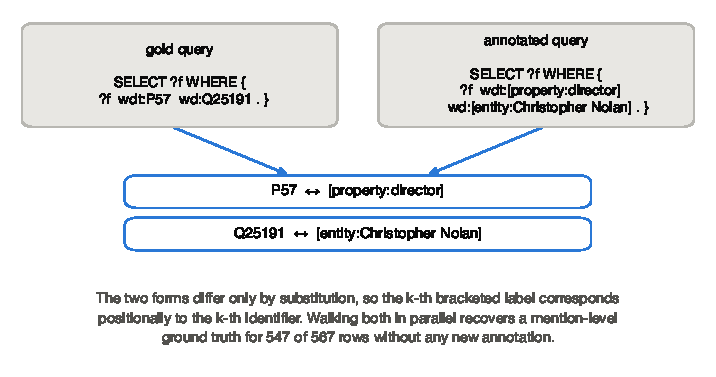
\includegraphics[width=0.88\textwidth]{figures/fig_groundtruth.pdf}
  \caption{Deriving mention-level linking ground truth from the benchmark.}
  \label{fig:groundtruth}
  \tabnote{Since the annotated query differs from the gold
query only through identifier substitution, alignment is positional and
requires no new annotation. It succeeds on 547 of 567 rows. The 20 rows
with different bracket and identifier counts are excluded for every
linker.}
\end{figure}

\section{Evaluation and Execution}

\subsection{Execution Environment}

\label{sec:setup-endpoint}

All queries are executed against a QLever instance provided by the AI \& Explainability group, indexing a Wikidata snapshot dated 14 March 2026; it was chosen because the rate limits and timeouts of the public Wikidata Query Service lowered execution success for reasons unrelated to query quality.
Three adaptations apply equally to reference and generated queries: the standard prefix block is added (QLever does not define it implicitly), \texttt{SERVICE wikibase:label} clauses are removed (they are Blazegraph-specific and affect only display labels, not the identifiers used for scoring), and responses are streamed with a 50 MB limit, above which they count as failures.
Execution failures are classified by cause (HTTP status, timeout, connection error, oversized result), as the stage analysis requires.

\paragraph{The Exclusion Taxonomy}

Of the 567 working test rows, 111 reference queries do not execute on QLever.
Of these, 26 also fail on the public endpoint (knowledge-graph evolution), and the remaining 85 fail for engine-specific reasons: Blazegraph's proprietary named-subquery extension, unavailable services (\texttt{wikibase:around}, \texttt{mwapi}, \texttt{gas}), timeouts, and queries that reuse a variable as an \texttt{AS} target (which QLever rejects as non-standard SPARQL while Blazegraph accepts it).
Approximately 15\,\% of reference queries are therefore Blazegraph-only; since generated queries face the same constraints, this does not bias the comparison between systems, but the evaluated subset is not a uniform sample of the full benchmark (see the limitations).

\subsection{Evaluation Metrics}

\label{sec:setup-metrics}

\paragraph{Result-Set Similarity and the Empty-Set
Artefact}

Accuracy is measured as the Jaccard similarity between the generated and reference result sets, after entity URIs are normalised to identifiers.
Two evaluation sets are used: the lenient set (456 of 567 working rows, wherever the reference executes) and the strict set, which additionally requires the reference to return at least one result (400 rows: 35 simple, 194 medium, 171 complex; these are \emph{scorable} counts, not the split's composition given above).
All headline results use the strict set.
It removes the first of the four metric problems examined in the discussion: the Jaccard similarity of two empty sets is 1.0, so among the 56 rows where the reference executes but returns nothing, a wrong generated query that also returned nothing scored perfectly, which inflated scores by two to seven points and changed model rankings in preliminary experiments.

\paragraph{Entity-Level Similarity as a Robustness
Check}

The pooled metric combines values across all result columns, so label mismatches lower it even when the underlying entities agree (about 16\,\% of end-to-end rows).
Entity-level Jaccard, which uses only identifiers, is therefore reported as well; it is up to six points higher and leaves the system ordering unchanged, which suggests that the pooled metric understates but does not distort the comparisons.
It is undefined when neither query returns entity values, so comparisons use the 316 strict rows where it is defined for every system (27 simple, 166 medium, 123 complex); full-set results are in the appendix.

\paragraph{Linking Metrics}

Linking is evaluated directly, because a query can fail structurally with every identifier correct, and one wrong identifier can spoil an otherwise correct query.
For each linker, precision, recall and F1 are computed over the predicted identifiers at mention level (exact match only; an unresolved mention counts against recall, not precision), together with the proportion of fully linked queries, broken down by complexity.
For ReFinED and ELQ, set-based precision, recall and F1 are computed as well (predicted versus reference identifier sets, without mention-level alignment), so the gap between mention-level and set-based scores estimates the effect of mention detection separately from disambiguation.

\paragraph{Construct-Agreement F1}

Usage counts alone cannot tell apart a system that never uses a construct from one that uses it constantly in the wrong places, and only the second is a calibration problem.
Construct-agreement F1 separates the two: with ``the reference query for question $q$ uses construct $C$'' as the positive class, it is the per-question F1 with which a system uses $C$ exactly where the reference does.
Because it is computed over query text rather than answers, knowledge-graph evolution does not affect it, and it stays meaningful even for rows whose reference no longer executes.

\paragraph{Statistical Testing}

Paired comparisons are reported with confidence intervals.
Prompt interventions and the cascade use paired bootstrap percentile intervals, a two-sided permutation test and the Wilcoxon signed-rank test; the linker comparison uses mention-level bootstrap resampling, applying the same resample to every linker in each iteration.
Complexity breakdowns and the comparison with the benchmark authors' systems are point estimates; differences below about one percentage point between neighbouring configurations are treated as ties, and the 27-row simple category in the common entity-level subset should be read with caution.

\section{Interventions and Failure
Recovery}

\subsection{Prompt Interventions}

\label{sec:method-prompts}

The error analysis in the results chapter identifies query structure as the main source of failure, in particular the underuse of constructs for qualified, quantified and hierarchical facts.
If this explanation is right, giving the model information about these constructs should improve generation.
Four prompt conditions test this.

All conditions use the same model, candidate pools, disambiguation backbone, execution environment and scoring; only the generation prompt changes.

\paragraph{Baseline.}

The model receives the task description given above: generate a query in bracket notation, keep ordinary SPARQL structure, and output only the query.

\paragraph{Idiom guidance.}

The baseline prompt is extended with seven rules about Wikidata modelling patterns.
They cover hierarchical class membership, statement nodes and qualifiers, value nodes for quantities, lexemes and forms, aggregation for counting and ranking, VALUES or UNION for alternatives, and avoiding unnecessary LIMIT clauses.
The model is told to apply only the constructs the question requires.
Each rule addresses a failure mode found in the error analysis, and the complete prompt is given in the appendix.

\paragraph{Schema evidence, verbose and
targeted.}

Generic guidance explains that a construct exists; schema evidence gives information about the entities and properties relevant to a specific question.
Following~\parencite{zhang2026saga}, the reference identifiers are probed against the endpoint to find their properties, qualifiers, class relationships and quantity values.
The information is presented in two forms:

\begin{itemize}
\item
A verbose card listing all retrieved information, averaging 329 words.
\item
A targeted card with conditional guidance for properties relevant to the question.

\end{itemize}

The cards are built from reference-linked mentions, not from the mentions the pipeline resolves.
This favours grounding, but the setting is not deployable because it relies on gold information, so it is treated as an upper-bound condition in the sense of the diagnostic protocol.

\subsection{Selective Application and the Execution-Guided
Cascade}

\label{sec:method-cascade}

The interventions raise a further question: can guidance be given only when it is needed?

\paragraph{Selective Application}

Unconditional idiom guidance can lead the model to overuse the constructs it describes.
A selective gate could predict whether a question needs a particular construct and include the matching rule only then, an approach also suggested by~\parencite{yang2026ggc}.

Such a gate must meet two conditions: the need for a construct must be predictable from the question, and the guidance must do harm when the construct is not needed.

To test predictability, a logistic-regression classifier is trained on unigram and bigram term-frequency features from the training split, with labels indicating whether the reference query uses the construct.
To test whether selective application could help, the effect of idiom guidance is measured separately for questions that do and do not need each construct.
An oracle gate then applies guidance only when the reference query requires a reification or hierarchy construct.
Because the oracle has access to the reference query, it represents the best possible gate, not a deployable system.

\paragraph{The Execution-Guided
Cascade}

The cascade relies on an observable failure signal instead of predicting the cause directly.
Every reference query in the evaluation set returns at least one result, so a generated query that executes but returns nothing must be wrong.

The cascade generates several queries for the same question with different prompts.
It executes them in a fixed order and accepts the first result set that is non-empty and free of execution errors (\cref{fig:cascade-mechanism}).

On this evaluation set, the method is monotonic.
It only replaces empty or failed results, which already score zero against a non-empty reference.
It needs no gold answers and no training.
A question whose first query fails is passed to the next prompt in the order, so it costs one further generation per fallback step; with the eight runs reported here, at most seven.

\begin{figure}[htbp]
  \centering
  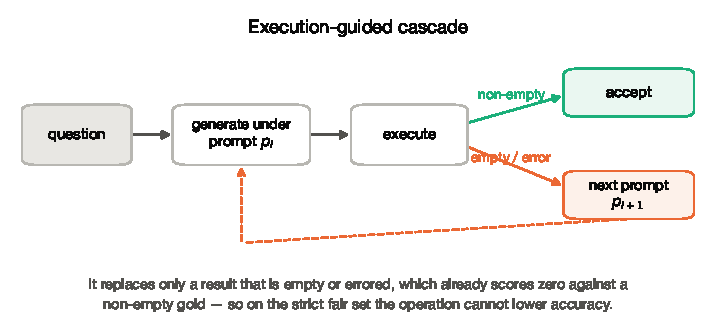
\includegraphics[width=0.88\textwidth]{figures/fig_cascade_mechanism.pdf}
  \caption{The execution-guided cascade.}
  \label{fig:cascade-mechanism}
  \tabnote{The trigger is similar to the execution feedback used by
agentic systems, but the cascade responds with a different prompt rather
than an open-ended self-correction loop. This limits the cost and
ensures monotonicity.}
\end{figure}

The cascade is compared with two alternatives that use the same candidates.
The first selects a result-set centroid: among the candidates that return results, it picks the one whose result set is, on average, most similar to the others.
The second adds a fallback to the best-performing single prompt when no candidates agree above a threshold.
These comparisons show whether the useful signal comes from agreement between candidate answers or simply from having a valid preferred result.

Execution feedback is established in mKGQAgent~\parencite{perevalov2025mkgqagent}, SPINACH~\parencite{liu2024spinach}, and GRASP~\parencite{walter2025grasp}.
These systems generally send execution failures back to the same prompt for revision.
A recent reinforcement-learning agent learns a policy for this revision step directly, training a compact model to recover from execution errors across turns~\parencite{vossebeld2025refine}.
The cascade instead switches to a different prompt for the same question, which limits the number of calls and makes it monotonic.

\section{Models and
Reproducibility}

\label{sec:setup-repro}

\paragraph{Models}

Four frozen frontier models are evaluated for generation: GPT-5.4, Claude Opus 4.8, Gemini 3.1 Flash Lite, and DeepSeek V4 Flash, accessed through the OpenRouter API with deterministic decoding, a 1,024-token limit, and up to three retries on empty responses.
The prompt-intervention arms, the official-split comparison and the Claude Opus 5 replication were run directly through Anthropic's API.
In the pipeline, Claude Opus 4.8 generates the labelled queries, except in the newer-model replication, which uses Claude Opus 5.
Claude Opus 4.8 also disambiguates in the working-split end-to-end run; the official-split run, the prompt-intervention arms and the Opus 5 replication disambiguate with Qwen2.5-14B-Instruct, and the backbone comparison varies the disambiguation model.
Qwen2.5-14B-Instruct and Qwen2.5-7B-Instruct are served through vLLM on the AI \& Explainability group's GPU server.

The seven prompt-intervention arms use Claude Opus 4.8 for generation and the same open-weight disambiguation model throughout, so the prompt is the only experimental variable.
This configuration was chosen because the experiment required seven complete pipeline runs, and it is supported by the backbone comparison, which shows similar disambiguation performance across backbones (97.7 entity F1 frontier vs.\ 94.9 and 95.8 open).
Absolute scores in these arms are therefore slightly lower than the frontier-disambiguated end-to-end results; comparisons within the arms remain valid, but absolute scores across sections should be read with this in mind.
The generator's identity was checked between arms through its lexical fingerprint (camelCase identifiers, snake\_case labels, bare property identifiers): all seven arms pass, while an open-backbone control run fails, which confirms that the check can detect a changed generator.

The official-split comparison differs in two respects: it uses Anthropic's batch interface, and it sets no temperature, since the API no longer supports this parameter for the model.
The two experiment sets should therefore not be compared at sub-percentage-point precision.

\paragraph{Caching, Re-Scoring, and Reproducibility}

Model outputs (generated queries, disambiguation decisions, substituted queries) are saved when they are generated; all later scoring, including the move from the public endpoint to QLever and every re-measurement after a correction, reuses these cached outputs instead of regenerating them, so differences between conditions cannot come from regeneration variance.
All reported numbers, tables and figures are recomputed from these stored outputs, as described in the appendix.
